% !TEX root = ../thesis.tex
% circle view of angular application
% @author Tobias Wulf
%

\section{Kreisdarstellung des klassischen Anwendungsfalls}\label{sec:kreisdarstellung-anwendung}


Im klassischen Anwendungsfall, zu sehen in \autoref{fig:klassischeranwendungsfall}, ist ein Gebermagnet räumlich 
zentriert über einen magnetischen Sensor platziert. Bei Drehung des Gebermagneten rotiert sein Magnetfeld entsprechend 
mit. Die Rotation findet um die $Z$-Achse des Gebermagneten statt. Die Nord-Süd-Ausrichtung des Magneten liegt in der 
$X$- bzw. $Y$-Achse des Koordinatensystems \cite{NXPSemiconductors2014}\cite{TDK2016}.
\newline
Der Winkelsensor misst, die zueinander und zur Rotationsachse orthogonal stehenden, $X$- und $Y$-Feldstärkenkomponenten 
des Gebermagneten $H_x$ und $H_y$. Diese setzt der Winkelsensor in elektrische Spannungssignale um. Die Winkelstellung 
$\alpha$ des Magnet wird somit nicht direkt gemessen. Sie kann aber, mittels der gemessenen $H_x$ und $H_y$ 
Feldstärkenkomponenten, durch einfache Vektorrechnung berechnet werden.
\newline
Bei idealer und gleichbleibender Position des Gebermagneten in Relation zum Winkelsensor, liefern die aufgenommen 
$H_x$-/ $H_y$-Messwerte eine Cosinus-Funktion $V_{cos}(H_x,H_y)$, sowie eine um $\SI{90}{\degree}$ zur Cosinus-Funktion 
phasenverschobene Sinus-Funktion $V_{sin}(H_x,H_y)$. Genaue physikalische Größenzusammenhänge und technische Umsetzung 
sind dabei vorerst in Darstellung vernachlässigt. 


\clearpage


\begin{figure}[tph]
	\centering
	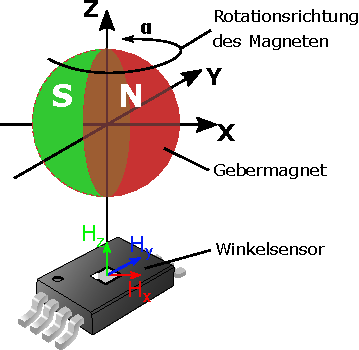
\includegraphics[width=0.35\linewidth]{chapters/images/2-Grundlagen/Klassischer_Anwendungsfall}
	\caption[Klassischer Anwendungsfall für die Drehwinkelerfassung]{Klassischer Anwendungsfall für die 
		Drehwinkelerfassung. Zeigt einen, um seine $Z$-Achse rotierenden, Gebermagneten und einen Winkelsensor in 
		zentrierter und orthogonaler Ausrichtung zur $Z$-Achse des Magneten. Idealerweise befinden sich Magnet und 
		Sensor, 
		ohne Verkippungen in $X$- oder $Y$-Richtung, parallel zueinander. Grafik entnommen und bearbeitet aus 
		\cite{Schuethe2020a}.}
	\label{fig:klassischeranwendungsfall}
\end{figure}


Durch die Phasenverschiebung der Sinus-Funktion stehen die Messwerte $V_{cos}(H_x,H_y)$ und $V_{sin}(H_x,H_y)$ 
vektoriell orthogonal zueinander. Bedingt durch die Orthogonalität der Messwerte $V_{cos}(H_x,H_y) \perp 
V_{sin}(H_x,H_y)$ und gleichförmige Kreisbewegung des Magneten um seine $Z$-Achse, beschreibt die Winkelmessung in 
polarer Darstellung eine konstante Kreisbahn. Diese besitzt einen konstanten Bahnradius $r$ und die Winkelstellung 
$\alpha$ des Gebermagneten \cite{Schuethe2019}.
\newline
Für eine beliebige Winkelmessung $\mathbf{A}$, die eine entsprechende Winkelstellung $\alpha$ des Gebermagneten 
abbildet $\mathbf{A}\mapsto\alpha$, ergibt sich somit folgender vektorieller Zusammenhang in \autoref{eq:vektorfeld} 
\cite{Schuethe2020}.


\begin{equation}\label{eq:vektorfeld}
\underbrace{\begin{pmatrix} H_x(\alpha) \\ H_y(\alpha) \end{pmatrix}}_{\textrm{Gebermagnetfeld}}\Rightarrow
\underbrace{
	\begin{pmatrix} V_{cos}(H_x,H_y) \\ V_{sin}(H_x,H_y) \end{pmatrix}}_{\textrm{Winkelsensormesswerte}}=
\underbrace{
	\begin{pmatrix} r\cdot\cos(\alpha) \\ r\cdot\sin(\alpha)\end{pmatrix}=
	\begin{pmatrix} a_x \\ a_y \end{pmatrix}}_{\textrm{Kreisdarstellung}}=
\underbrace{\mathbf{A}(\alpha) \vphantom{\begin{pmatrix}x\\y\end{pmatrix}}}_{\textrm{Winkelmessung}}
\end{equation}

Die so erhobenen Winkelmessung $\mathbf{A}$ nach \autoref{eq:vektorfeld}, bildet ein eindimensionales Vektorfeld mit 
$\{a_x,b_x\}\in\mathbb{R}$ ab. Wobei sich der Bahnradius $r$ für die Kreisdarstellung, aus dem Betrag der Messung 
$|\mathbf{A}|$, nach \autoref{eq:bahnradius} gewinnen lässt.


\begin{equation}\label{eq:bahnradius}
r = |\mathbf{A}| = \sqrt{\big(V_{cos}(H_x,H_y)\big)^2 + \big(V_{sin}(H_x,H_y)\big)^2} =\sqrt{a_x^2 + a_y^2}
\end{equation}


\clearpage


\begin{figure}[tph]
	\centering
	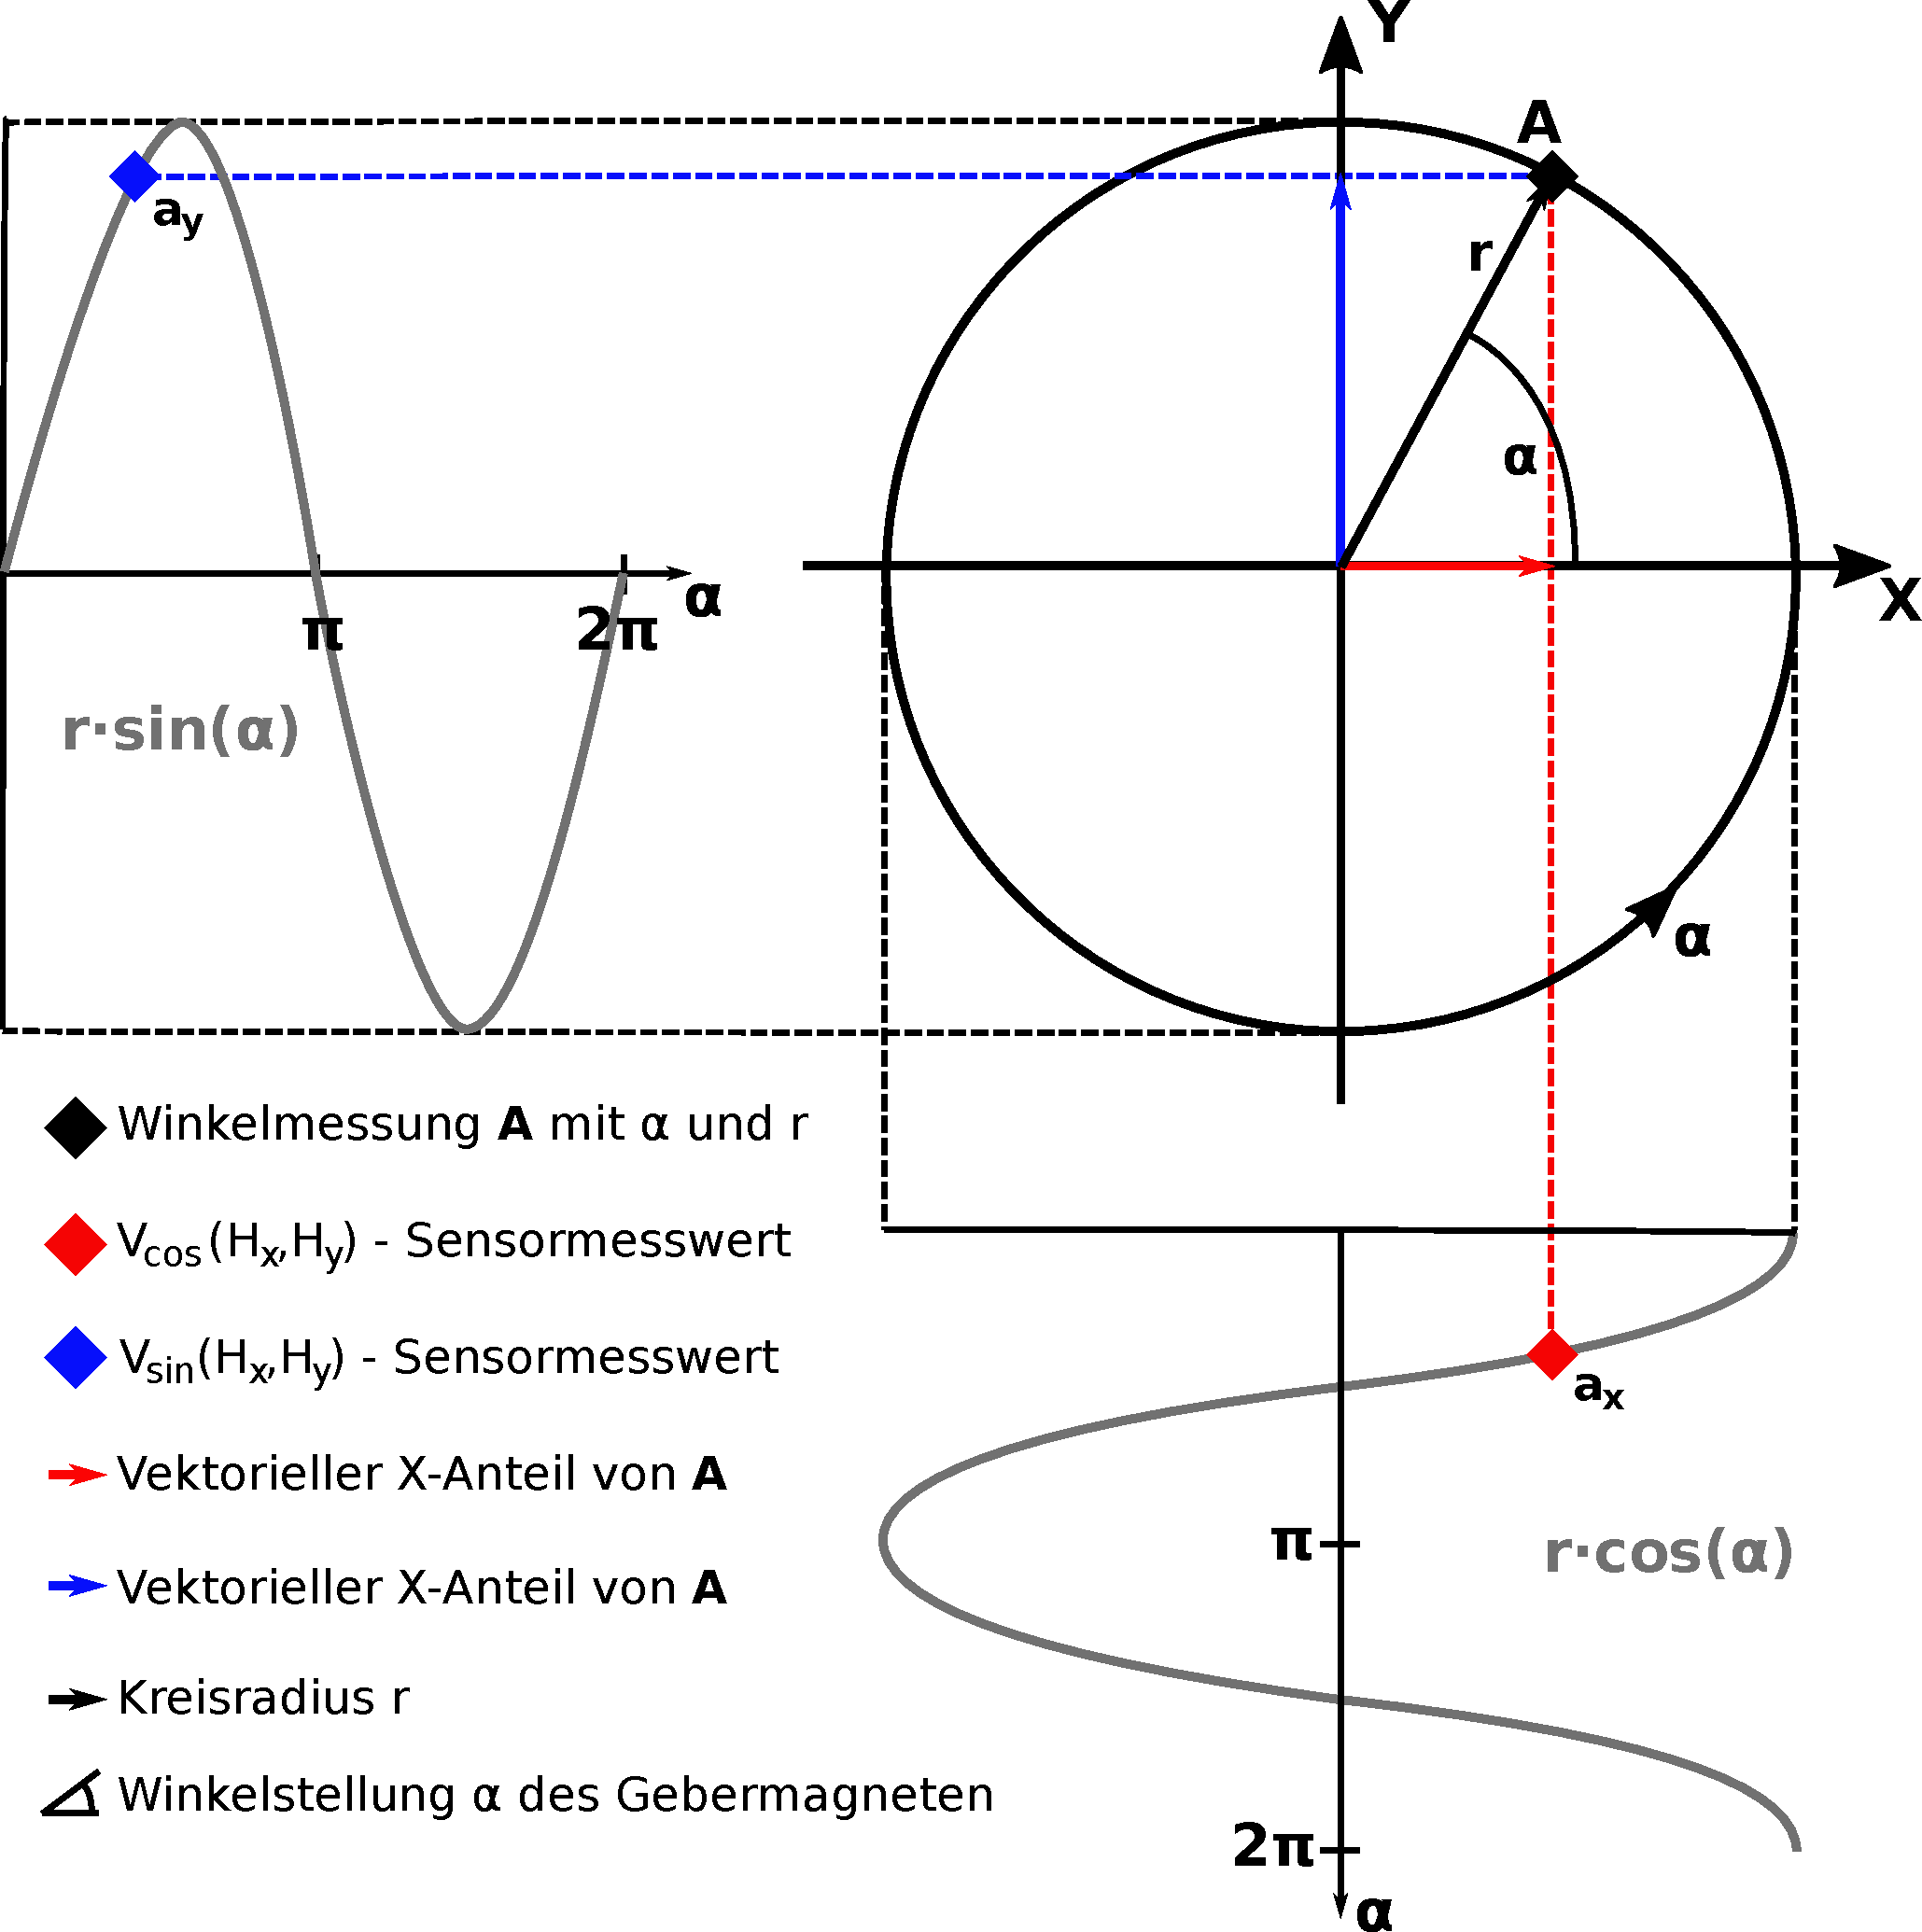
\includegraphics[width=0.7\linewidth]{chapters/images/2-Grundlagen/Kreisdarstellung_Winkelmessung}
	\caption[Kreisdarstellung der Winkelmessung]{Kreisdarstellung der Winkelmessung. Als Abbildung der
		Winkelmessung $\mathbf{A}\mapsto\alpha$ aus	\autoref{eq:vektorfeld}. Die Zusammensetzung der Messung erfolgt 
		durch, die vom Winkelsensor gemessenen, vektoriellen Anteile für die polare Darstellung der 
		Gebermagnetwinkelstellung.}
	\label{fig:kreisdarstellungwinkelmessung}
\end{figure}

Der entsprechende Winkel des Gebermagneten lässt sich, mittels Überführung in Polarkoordinaten, nach \autoref{eq:atan2} 
zurückrechnen. Die \autoref{fig:kreisdarstellungwinkelmessung} veranschaulicht den Zusammenhang zwischen Messwerten und 
Abbildung der Gebermagnetwinkelstellung. Die Sinoiden Messergebnisse sind der $\text{arctan2}$ Funktion zuzuführen. 
Diese bildet einen Winkel von null bis $\pi$ ab und besitzt eine Sprungstelle bei $\pi$. Der $Y$-Anteil kann dabei 
als Entscheider genutzt werden, um eine Abbildung des Winkels auf eine volle Kreisumdrehung $(2\pi)$ umzusetzen. 


\begin{equation}\label{eq:atan2}
\alpha = 
	\begin{cases}
	\text{arctan2}(a_y,a_x)        &\quad \textrm{f. } a_y > 0 \\
	\pi							   &\quad \textrm{f. } a_y = 0 \\
	\text{arctan2}(a_y,a_x) + 2\pi &\quad \textrm{f. } a_y < 0
	\end{cases}
\end{equation}
